\documentclass[12pt,a4paper]{book}
\usepackage[latin1]{inputenc}
%\usepackage{cclicenses}
\usepackage{url}
\usepackage{amsmath}
\usepackage{amsfonts}
\usepackage{amssymb}
\usepackage{graphicx}
\usepackage{multicol}
\setcounter{tocdepth}{1}
\author{Paul Sutton}
\begin{document}

\begin{center}
{\Huge ToriOS Manual}
\end{center}
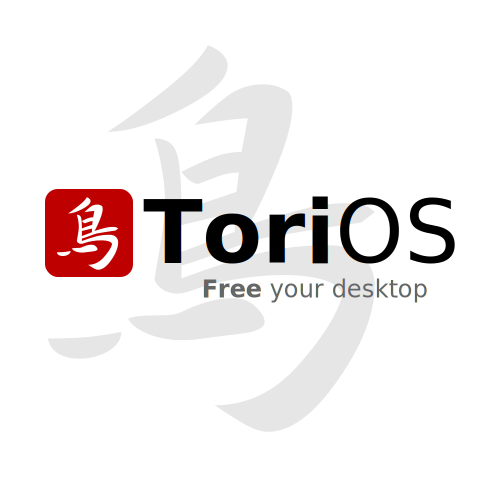
\includegraphics{FinalLogo}

\begin{center}
Minimal, Simple, Fast, Small and Gives you a freedom of choice :)
\end{center}
\tableofcontents
\chapter{Introduction}
The goal of this project is to produce a minimalist Linux distribution that gives end users more choice as to what software is installed on their system.\\

Ubuntu 12.04 is used as a base for this new system.
\subsection{About this Manual}
This manual refers to external websites to help explain concepts further, to avoid the need to reproduce what is already out there.  The ToriOS team take no responsibility for external content.  The links are correct and suitable at the time of writing,  Broken links are out of the Authors control between revisions.  It is your responsibility to ensure suitability of information, you should read fully and seek other sources of information and ask for help if unsure.  
This manual has been prepared using \LaTeX. 

\chapter{What is GNU / Linux}


\subsection{About ToriOS}

ToriOS is a system aimed at replacing Windows XP, which will reach end-of-life in April 2014. ToriOS is a fast and minimal system based on Ubuntu 12.04. 
\subsection{Non PAE Support}

ToriOS will support PAE Hardware\\
https://blueprints.launchpad.net/torios/+spec/non-pae-support

\subsection{Technical overview}

\begin{enumerate}
\item 1- ToriOS is supporting Non-PAE machines by default - we have already agreed on that - just a reminder.
\item 2- ToriOS is always an LTS - we too agreed on that as well - just a reminder.
\item3- ToriOS will be released every 12 months NOT every 6 months like Ubuntu - new idea.
\item4- ToriOS 1.0 is based on 12.04 LTS - we have discussed that before but didn't yet 100% agree on.
\item5- ToriOS 2.0 will be based on 14.04 LTS
\item6- nm-manager should not be used as far as I have read so far from different people all of them confirmed the big RAM eater is nm-manager.
\item7- While we're targeting low hardware machines (32-bit), shouldn't we also think of those who wish to try ToriOS on more powerful machine (64bit)? if that so, we need two builds: i386 and amd64.
\item8- I need the Wiki and Docs team to write each and every post, not only about the system, how to use it, system requirement, etc ... no ... I'm planning to document the steps that we have done to create this or will create this system and YES, I mean the technical side so I guess both the docs and devs guys need to work side by side if you agree on this.
\item9- 60MB or 50MB? don't want to kill ourselves but if we could do that, why not? I guess you know what I'm talking about
\item 10- Have we thought about the ISO size? any idea how big will it be? around 300MB? 400MB? less or more? AFAIK, it should never reach say 600MB, right?
\item 11- Where are we going to host the ISOs? do we have a host for that?
\item 12- As long as ToriOS is based on Ubuntu, we can test it on Virtual Machine such as OracleVB, correct?
\item 13- By any chance, do we need to talk with Ubuntu/Canonical team about our Project? I mean is there any kind of approval or stuff like that we need? I'm talking about the technical side of our project as they should have nothing to do with the other stuff but maybe they do with the technical side, that is why I'm asking and we need to know IMHO.
\item 14- Alpha 1, Alpha 2, Beta 1, Beta 2 and RC? or no need for that? should we just do Alpha, Beta and RC? these are milestones just like what Ubuntu GNOME or Lubuntu are doing when it comes to the development cycle.
\item 15- I know it is hard to tell at this point but any idea when ToriOS 1.0 will be available to download and use? I know I'm the one who should announce that but if truth to be told, it is something that our devs should advise for and we haven't yet done anything serious. 
\end{enumerate}

\chapter{The ToriOS Team}

\begin{tabular}{|c|c|c|c|c|}
\hline  \textbf{JOB \ ROLE} & \textbf{NAME}  & \textbf{IRC NICK} & \textbf{E-MAIL}  \\ 
\hline  Project lead & Ali Linx  & amjjawad & amjjawad@torios.org  \\ 
\hline  Website email admin & William  & ? & william@torios.org  \\ 
\hline  Documentation (manual)  & Paul Sutton  & zleap  & zleap@torios.org \\ 
\hline  Documentation (wiki) & Geoffrey De Belie & smile  & smile4ever@torios.org  \\ 
\hline  Developer lead / driver & Alexander Kluth & DerAlex & alexander@torios.org \\ 
\hline  QA Testing & Jack  & fjack  &  \\ 
\hline  Marketing & David &  & dbyentzen@AT@torios.org \\
\hline Artwork & Rafael & rafeallaguna & \\
\hline ? & Israel & israeldahl & \\

\hline 
\end{tabular}


\chapter{Installation}
\subsection{Downloading the ISO}
\subsection{Verifying the download}
There is an excellent guide at\\ \textbf{https://help.ubuntu.com/community/HowToMD5SUM} \\
that explains how to check your downloaded iso file for errors.  Apart from the file name being different so for ToriOS you may have ToriOS-1.0.0.iso the steps are pretty much the same.  
\subsection{Creating install media}
\subsection{booting install media}
Depending on how your computer is set up,  you need to tell the computer to boot of which ever boot media you created either a) cdrom b) dvd c) usb.

\subsection{UEFI Boot}
If you have very new hardware then you may have the new UEFI boot system,  this means you can't just boot the install media and there are a few extra steps.  These are outlined here.
\subsection{Installing}
\subsection{Final steps}
\chapter{Desktop}

ToriOS will use the JWM (Joe's Window Manager) window environment:\\

The following is quoted from the projects website

\begin{quote}
JWM is a light-weight window manager for the X11 Window System. JWM is written in C and uses only Xlib at a minimum. Because of its small footprint, JWM makes a good window manager for older computers and less powerful systems, such as the Raspberry Pi, though it is perfectly capable of running on modern systems. JWM is included in small Linux distributions such as Puppy Linux and Damn Small Linux, and it is available as a separate package in many other distributions. 
\end{quote}
http://www.joewing.net/projects/jwm/

\chapter{Applications}

\chapter{Get Involved}



\begin{itemize}
\item{Create a Launchpad Account [1]}
\item{Join the Team [2]}
\item{Subscribe to mailing list [3]}
\item{Send an e-mail to the list to introduce yourself}
\item{Choose where you would like to help [4]}
\end{itemize}

\begin{enumerate}
\item {https://help.launchpad.net/YourAccount/NewAccount}
\item {https://launchpad.net/~torios}
\item {https://help.launchpad.net/Teams/MailingLists - see subscribing}
\item {https://blueprints.launchpad.net/torios/+spec/recruit-contributors}

\end{enumerate}

\url{https://www.youtube.com/watch?v=P_r2hHqyUa4}
\url{http://www.youtube.com/watch?v=PtVxDv_vy8w}

\chapter{Glossary}
\begin{multicols}{2}


\begin{description}
\item[A]
\item[B]
\item[C]
\item[Creative commons] Document and Graphics Licensing.
\item[D]
\item[E]
\item[ext(n)] File system used on Linux systems, examples are ext2 ext3, and ext4 
\item[F]
\item[G]
\item[GPL] General Public License 
\item[GNU/LINUX] The kernel is released under the GPL so we refer to it as GNU / Linux
\item[H]
\item[I]
\item[J]
\item[K]
\item[Kernel] This is the heart of the operating system.
\columnbreak
\item[L]
\item[Linux] Operating system Kernel. 
\item[Linus Torvalds] Creator of the Linux Kernel
\item[M]
\item[N]
\item[O]
\item[P]
\item[PAE Hardware] Physical Address Extension 
\item[Q]
\item[R]
\item[S]
\item[T]
\item[U]
\item[V]
\item[W]
\item[X]
\item[Y]
\item[Z]
\end{description}
\end{multicols}
\chapter{Document License}

%\cc \ccby \ccsa



\end{document}